% Very simple template for lab reports. Most common packages are already included.
\documentclass[a4paper, 11pt]{article}
\usepackage[utf8]{inputenc} % Change according your file encoding
\usepackage{graphicx}
\usepackage{url}
\usepackage{listings}
\usepackage{xcolor}

% Configure listings for Erlang code
\lstdefinestyle{erlang}{
    language=erlang,
    backgroundcolor=\color{gray!10},
    basicstyle=\ttfamily\small,
    breaklines=true,
    frame=single,
    numbers=left,
    numberstyle=\tiny,
}

%opening
\title{Report 1: Rudy the HTTP Server}
\author{Lorenzo Deflorian}
\date{\today{}}

\begin{document}

\maketitle

\section{Introduction}

\textit{Summary of the work you've done, what are the topics we cover
  in this seminar, etc. Remember that you should deliver this report
  at the start of the seminar.}

The main goal of this assignment was to implement a simple HTTP server using Erlang. 
The server had to be able to receive connections from a socket, parse the HTTP request and send back an answer.
Another important aspect was to understand more about Erlang processes and how to use them to handle multiple clients concurrently.
Finally I had to evaluate the performance of my server comparing the different implementation approaches I explored.


\section{Main problems and solutions}

\textit{Summarize your problems, proposed solutions, etc. You do not
  need to copy\&paste your code. Only if needed, you may write down
  small code snipeds to show how you have solved a specific
  problem/question.}

The first task was to create a simple HTTP server that could handler requests sequentially.
This was quite straightforward using the built-in \texttt{gen\_tcp} module to handle socket connections. Once I implemented the basic server, I did a benchmark to see how it performed handling 100 requests sequentially.

\begin{lstlisting}[style=erlang, caption={Benchmarking the sequential server}]
(client@DORORO)1> test:bench(localhost, 8080).
Time Elapsed 174.338 ms
ok
\end{lstlisting}

Normalizing the time elapsed by the number of requests, I got an average latency of 1.743 ms per request. Hence our server is able to handle around 573 requests per second.

The next step was to add a small processing delay (40 ms) to simulate a more realistic scenario and see if the overhead given by the parsing of the request is significant.

\begin{lstlisting}[style=erlang, caption={Benchmarking the sequential server with processing delay}]
(client@DORORO)1> test:bench(localhost, 8080).
Time Elapsed 4408.464 ms
ok
\end{lstlisting}

The artificial delay radically increases the latency time to 44 ms per request, showing that the overhead of the server is negligible compared to the processing time.

\section{Evaluation}

\begin{figure}[h]
  \centering
  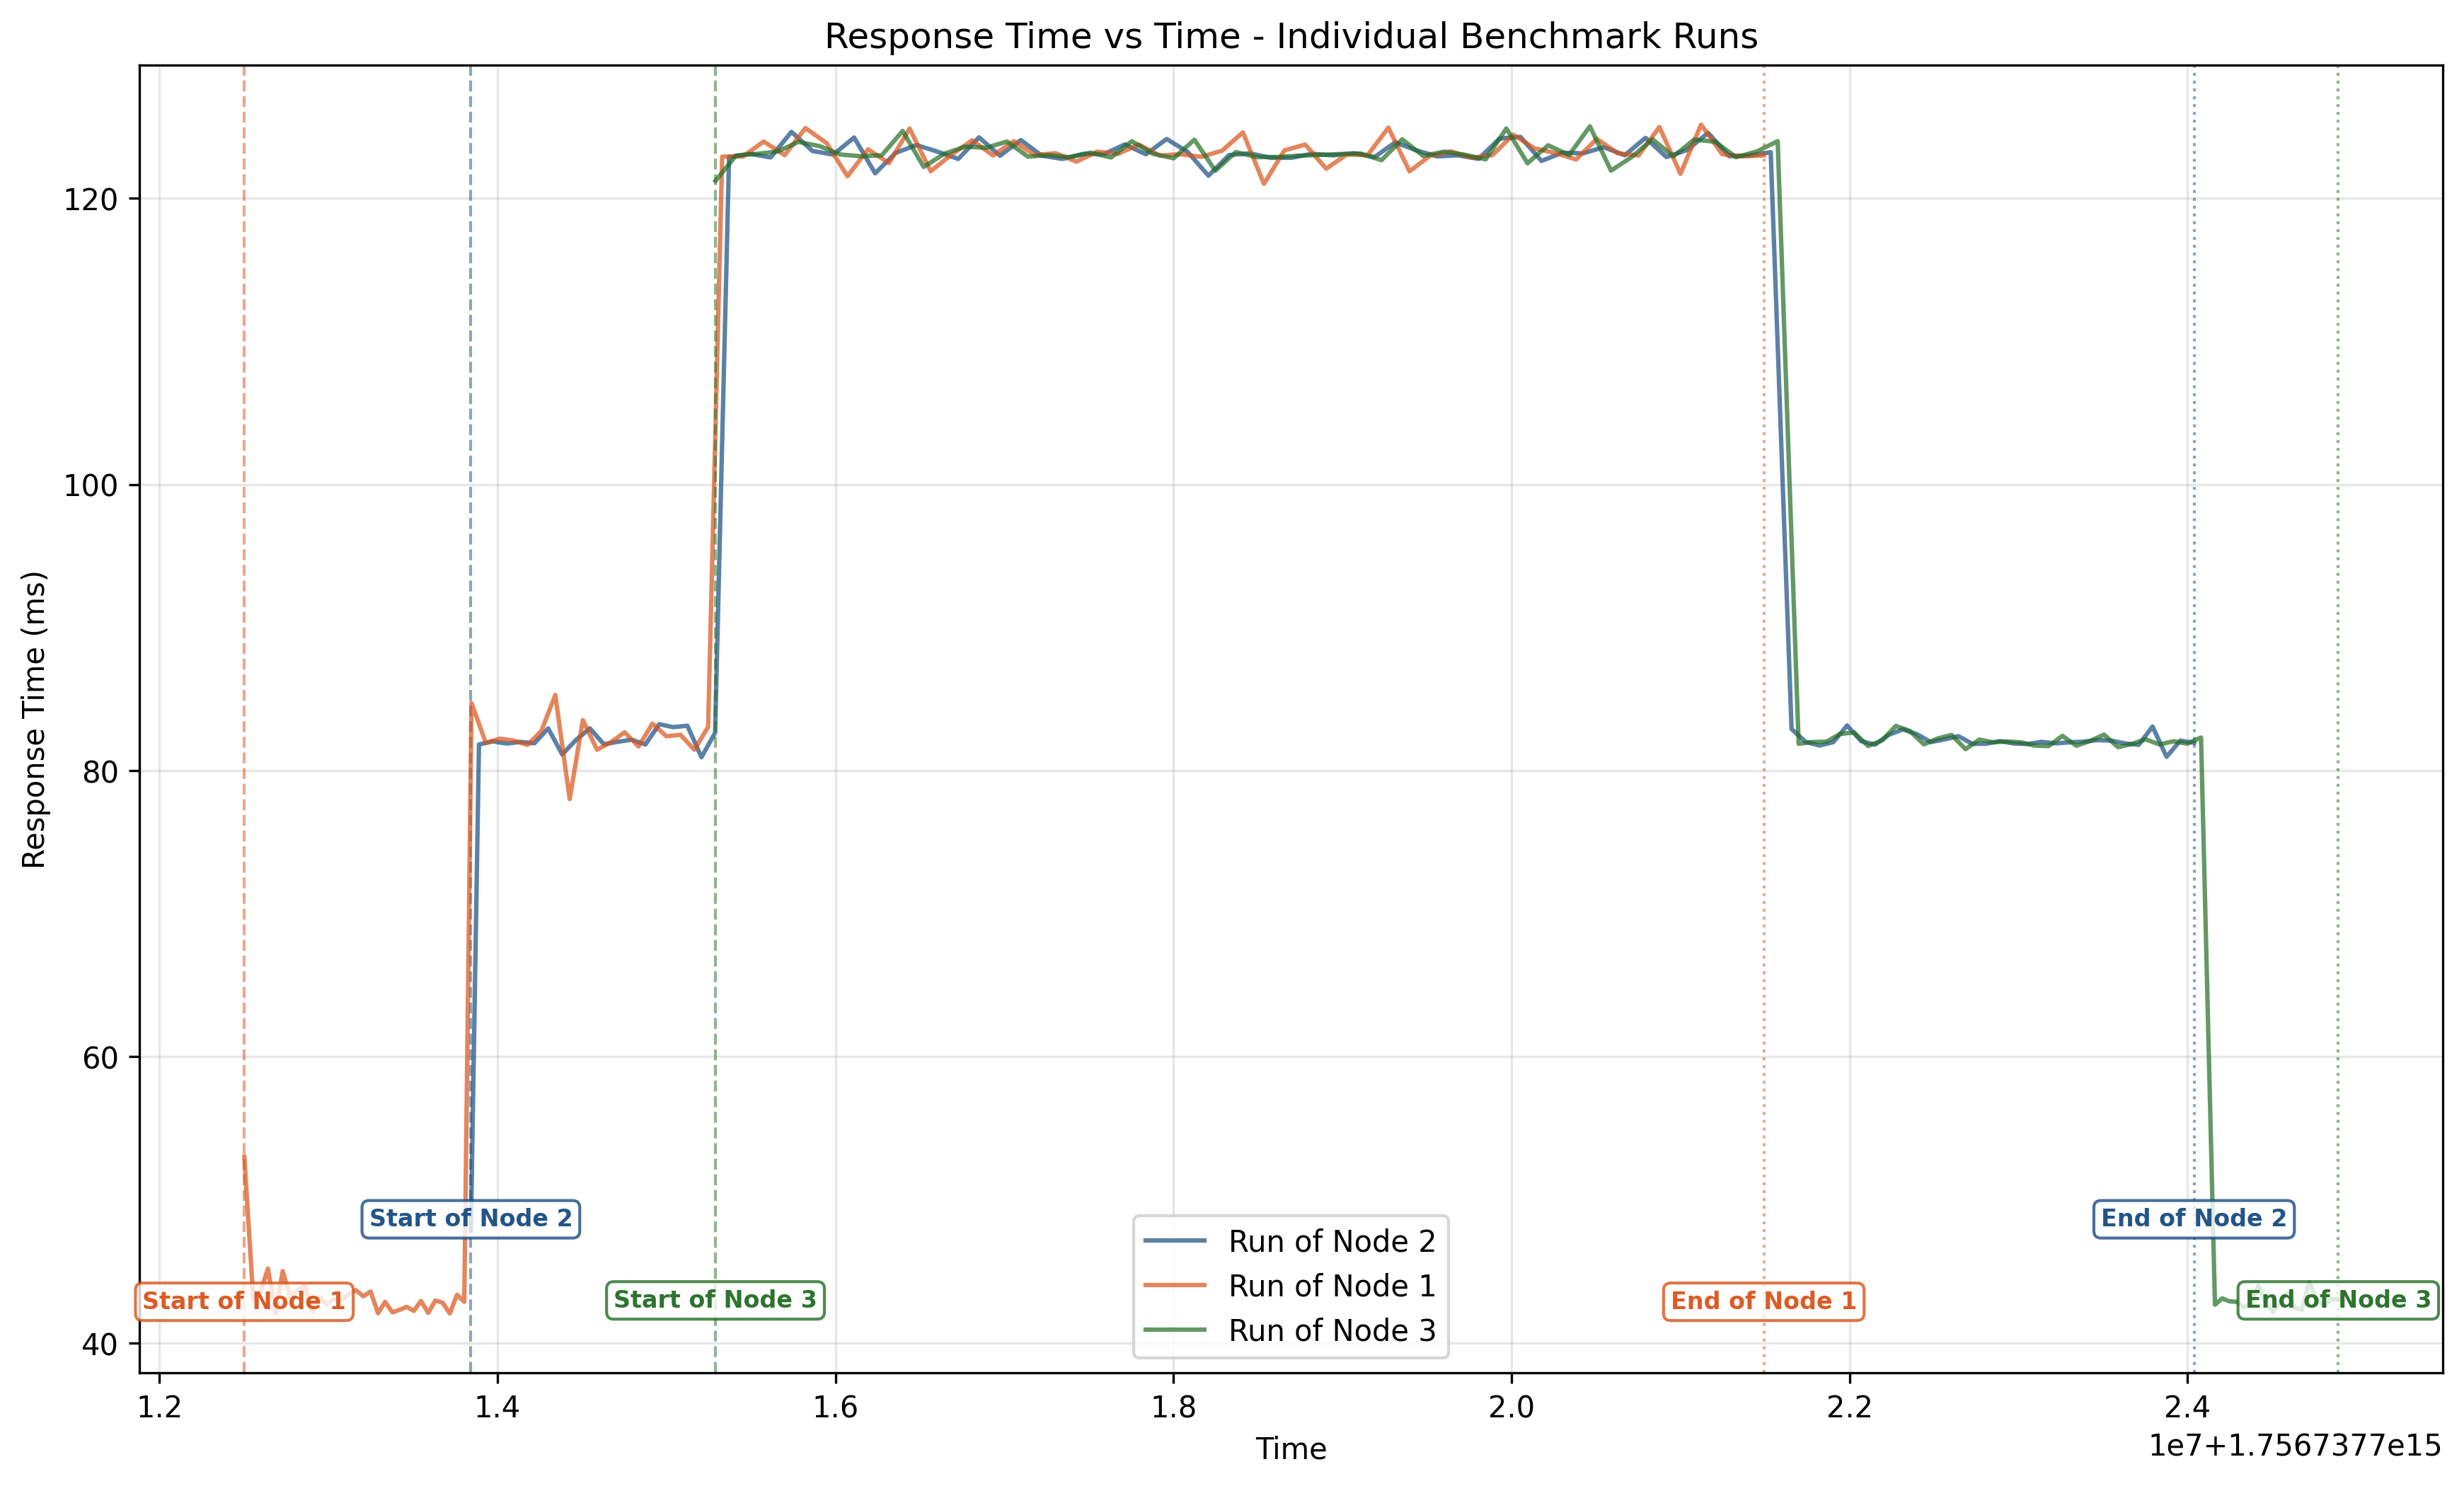
\includegraphics[width=0.9\linewidth]{sequential_benches/latency_plot.png}
  \caption{Latency Comparison (Sequential)}
  \label{fig:latency_comparison_seq}
\end{figure}

\begin{figure}[h]
  \centering
  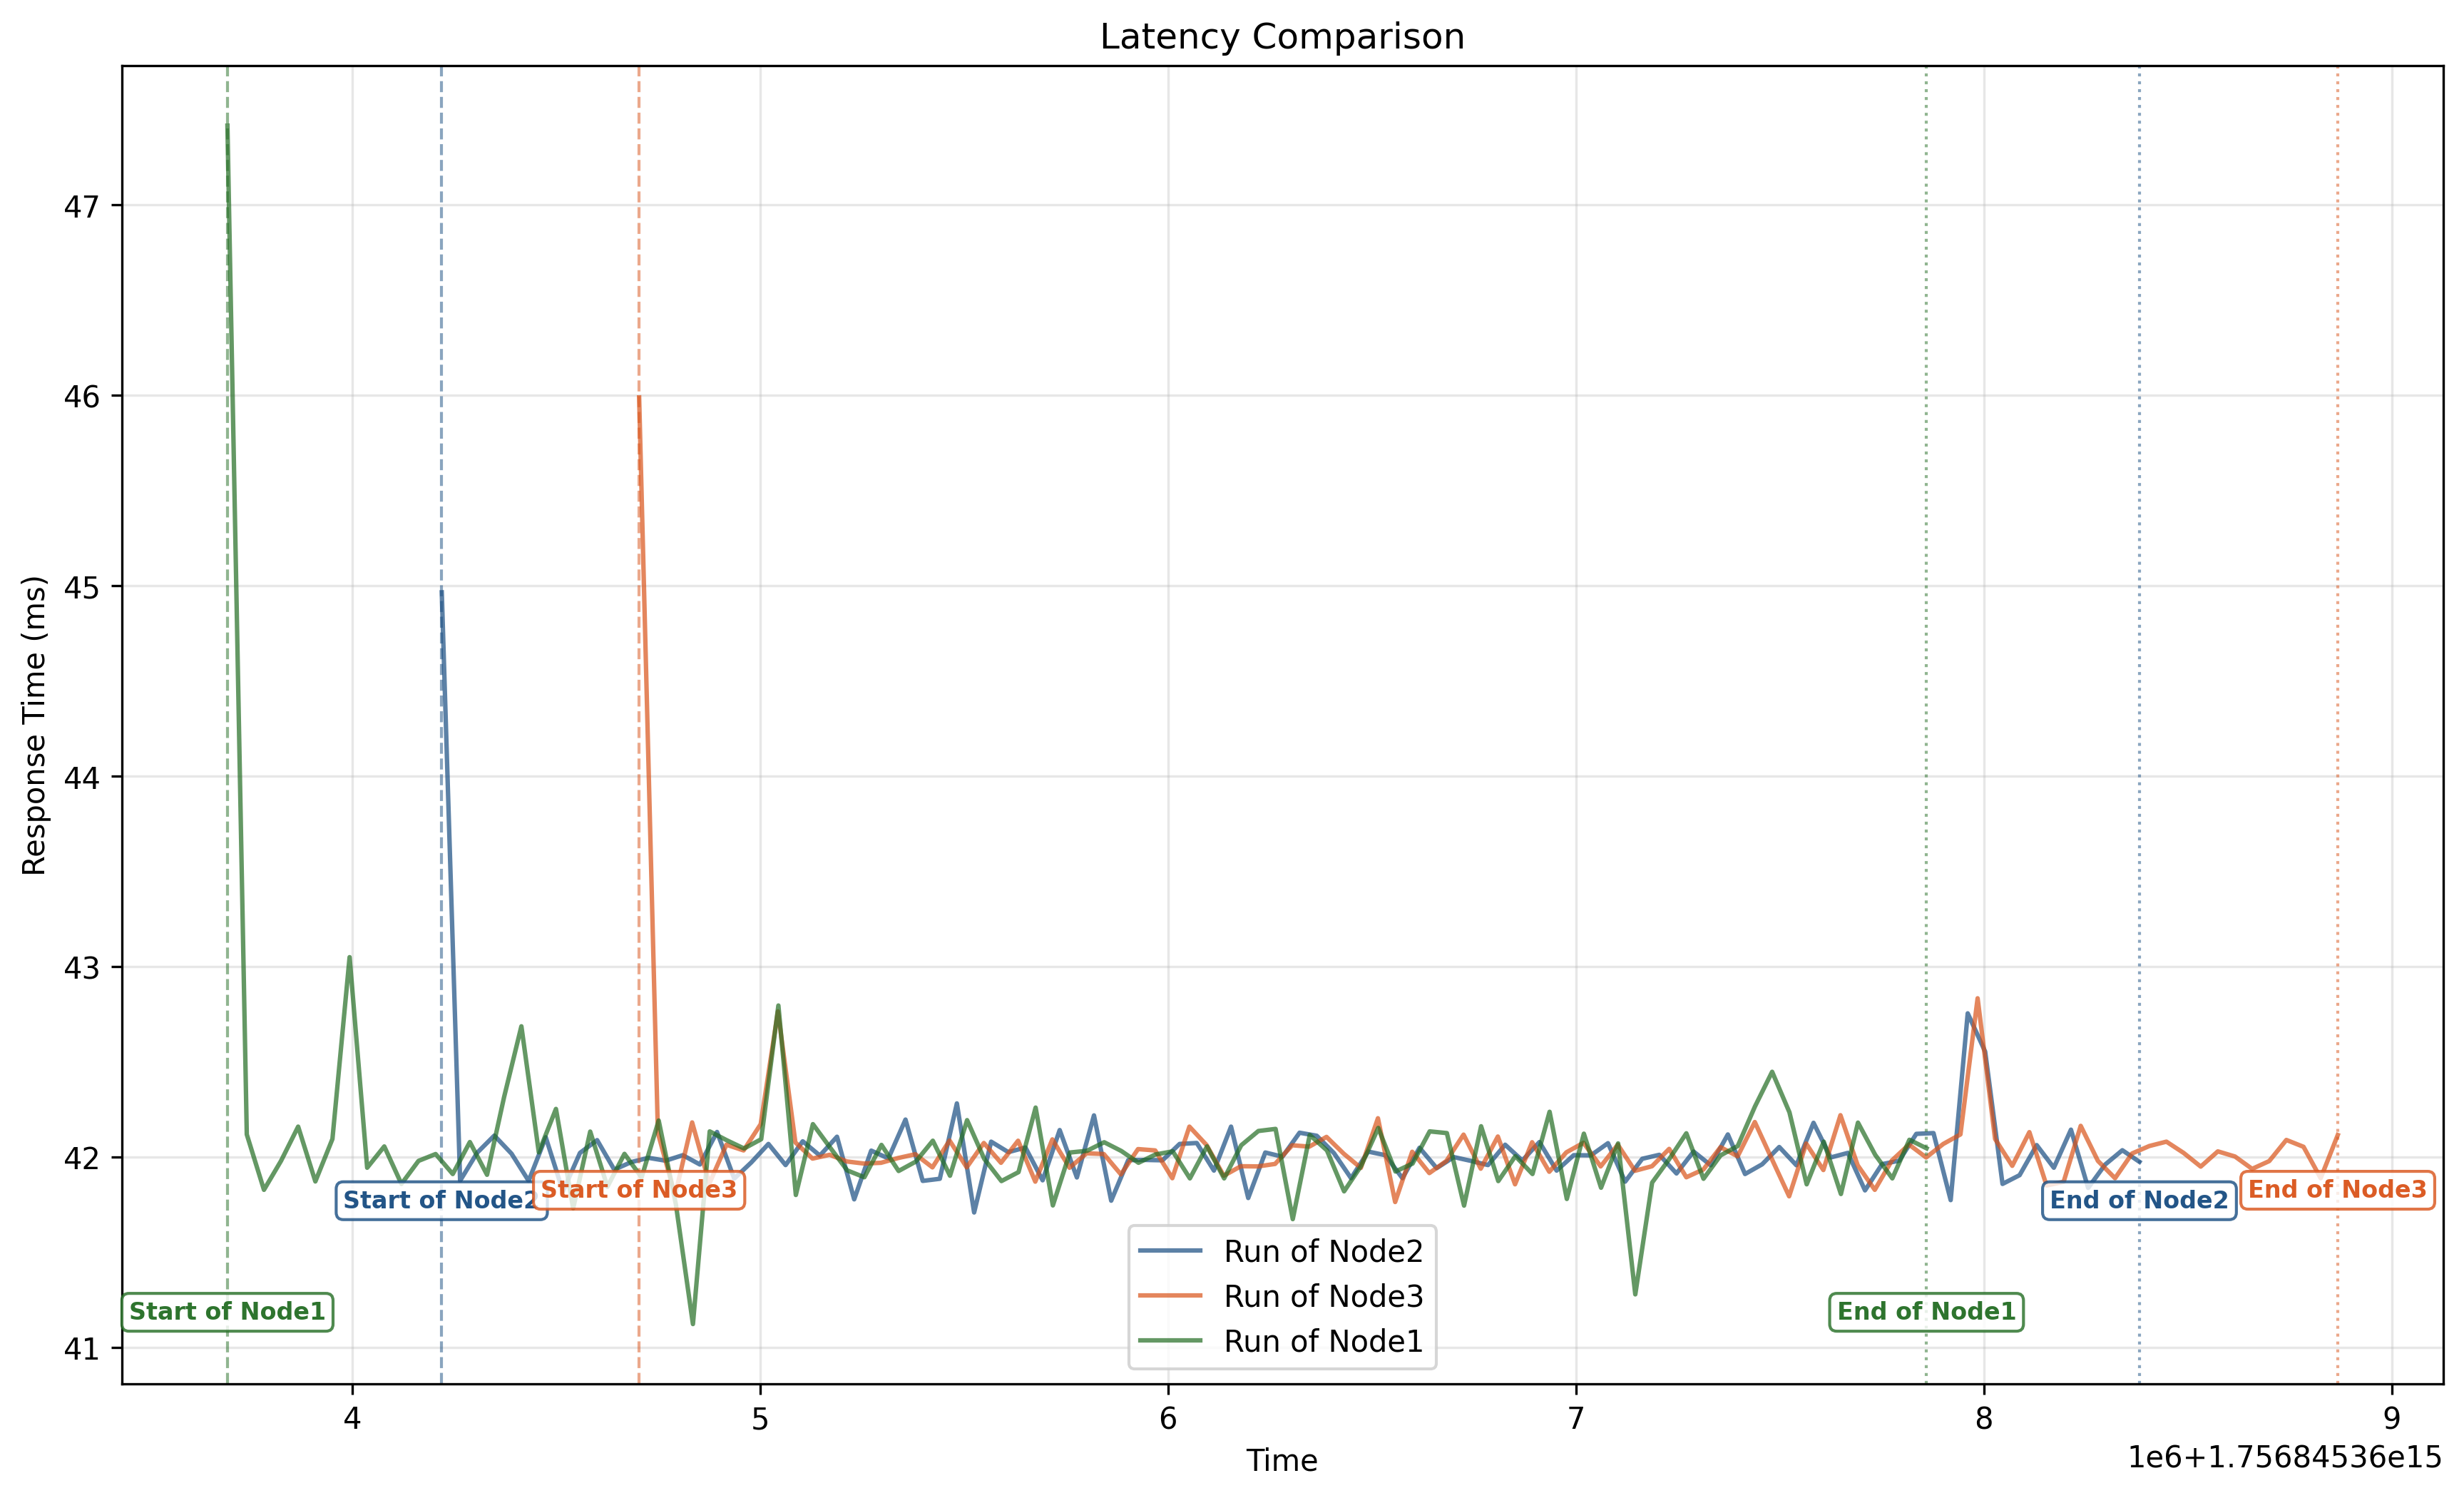
\includegraphics[width=0.9\linewidth]{concurrent_benches/latency_plot.png}
  \caption{Latency Comparison (Concurrent)}
  \label{fig:latency_comparison_conc}
\end{figure}


\section{Conclusions}

\textit{Change the layout of this template as you want. It's only for
  your guidance but if you feel that you need a different structure,
  feel free to change it. The report should not be too long ($\approx$
  2-3 pages).}

What have you learnt from the problem presented?
Was it useful?


\end{document}